\subsection{Study of Neutrino Freeze-out using the Boltzmann-Einstein Equation}\label{ch:param:studies}
%%%%%%%%%%%%%%%
In this section we remove the instantaneous freeze-out assumption and present results of a more precise study of neutrino freeze-out\index{neutrino!freeze-out}: We do not assume that the distribution is either in chemical or kinetic equilibrium or is free-streaming. The required mathematical theory and numerical method is developed in Appendices \ref{ch:vol:forms}, \ref{ch:boltz:orthopoly}, and \ref{ch:coll:simp}. Here we focus our attention on the physical implications, in particular the dependence of the freeze-out process on natural constants. This allows us identify potential avenues by which the tension between observed in terms of present day value of Hubble paramter $H_0$ and the related theoretical value of $N^{\mathrm{eff}}_\nu$, the key feature of the invisible today neutrino background, may be alleviated. 

Our study also constrains the time and/or temperature variation of certain natural constants by comparing the results with measurements of $N_\nu^{\mathrm{eff}}$. Further details on this work were presented in~\rsec{sec:model:ind},  more details can be found in Ref.\,\cite{Birrell:2014uka}. The topic of the time variation of natural constants is a very active field with a long history; for a comprehensive review of this area, with which we make only slight contact, see {\it e.g.\/} Ref.\,\cite{Uzan:2010pm}. 

%%%%%%%%%%%%%%%%%%%%%%%%%%%%%%%
\para{Neutrino Freeze-Out Temperature and Relaxation Time} 
To connect with the instantaneous freeze-out model from \rf{sec:model:ind}, we now give a definition of the kinetic freeze-out temperature that is applicable to the Boltzmann-Einstein equation model and use this to calculate the neutrino freeze-out temperature. Any such definition will be only approximate, as the freeze-out process is not a sharp transition. Our definition is motivated in part the treatment in \cite{Kolb:1990vq}. 

We first define a characteristic length between scatterings. Using the formula \req{n:div}, we obtain the fractional rate of change of comoving particle number
\begin{align}
\frac{\frac{d}{dt}(a^3 n)}{a^3n}=\frac{g_\nu}{2\pi^2n}\int C[f]p^2/Edp\,.
\end{align}
Here we don't want the net change, but rather to count the number of interactions. For that reason, we imagine that only one direction of the process is operational and define the relaxation rate\index{relaxation rate}
\begin{align}
\Gamma\equiv\frac{g_\nu}{2\pi^2n}T^2\int \tilde C[f]zdz\,,
\end{align}
where the one way collision is $\tilde C[f]$ is computed as in \req{coll} except with $F$ replaced by 
\begin{equation}
\tilde F=f_1(p_1)f_2(p_2)f^3(p_3)f^4(p_4)\,.
\end{equation}
If particle type $1$ also participates in the reverse of the reaction $1+2\rightarrow 3+4$ then a corresponding term for the reverse reaction must also be added. The key difference is there is no minus sign; here we are counting reactions, not net particle number change.

Using the average velocity, which for (effectively massless) neutrinos is $\bar v=c=1$, we obtain what we call the scattering length\index{scattering length}
\begin{align}
L_\Gamma&\equiv\frac{\bar v}{\Gamma}=\frac{\int_0^\infty\frac{1}{\Upsilon^{-1}e^z+1}z^2dz}{\int_0^\infty \tilde C[f] z^2/E dz}\,.
\end{align}
This can be compared to the Hubble length $L_H=c/H$\index{Hubble!length} and the temperature at which $L_\Gamma=L_H$ we call the freeze-out temperature\index{freeze-out!temperature} for that reaction. Figure \ref{fig:scattLength} shows the scattering length and $L_H$ for various types of neutrino reactions. The solid line corresponds to the annihilation process $e^+e^-\rightarrow \nu\bar\nu$, the dashed line corresponds to the scattering $\nu e^\pm\rightarrow \nu e^\pm$, and the dot-dashed line corresponds to the combination of all processes involving only neutrinos. The freeze-out temperatures in MeV are given in Table \ref{table:freezeoutTemp}.

\begin{table}[ht]
\centering 
\begin{tabular}{|c|c|c|c|}
\hline
 & $e^+e^-\rightarrow \nu\bar\nu$ & $\nu e^\pm\rightarrow \nu e^\pm$ & $\nu$-only processes\\
\hline
$\nu_e$ &2.29 & 1.15&0.910\\
\hline
$\nu_{\mu,\tau}$ &3.83 & 1.78& 0.903\\
\hline
\end{tabular}
\caption{Freeze-out temperatures in MeV for electron neutrinos and for $\mu$,$\tau$ neutrinos.}
\label{table:freezeoutTemp}
\end{table}

%%%%%%%%%%%%%%%%%%%%%%%%%%%%%%%%%%%%%%%
\begin{figure} 
\centerline{\includegraphics[width=0.82\linewidth]{04-birrell/ParametricStudies/Figures/nu_e_scattering_length_eta_0_23.pdf}}
\centerline{\includegraphics[width=0.82\linewidth]{04-birrell/ParametricStudies/Figures/nu_mu_scattering_length_eta_0_23.pdf}}
\caption{Comparison of Hubble parameter to neutrino scattering length for various types of PP-SM processes, top for electron neutrino $\nu_e$ and bottom for the other two flavors $\nu_\mu$, $\nu_\tau$. \cccite{Birrell:2014uka} }\label{fig:scattLength}
\end{figure}
%%%%%%%%%%%%%%%%%%%%%%%%%%%%%%%%%%%%%%%


We now consider the the relaxation time\index{relaxation time} for a given reaction, defined by $\tau=1/\Gamma$. Suppose we have a time interval $t_f>t_i$ and corresponding temperature interval $T_f<T_i$ during which there is no reheating and the Universe is radiation dominated. Normalizing time so $t=0$ corresponds to the temperature $T_i$ we have
\begin{equation}\label{ch6:Heq}
\dot a/a=-\dot T/T\,,\hspace{2mm} H=\frac{C}{2Ct+T_i^2}\propto T^2
\end{equation}
where $C$ is a constant that depends on the energy density and the Planck mass. Its precise form will not be significant for us. Note that \req{ch6:Heq} implies
\begin{equation}
1/H(t)-1/H(0)=2t\,.
\end{equation}

At $T\gg m_e$, the rates for reactions under consideration from Tables \ref{table:nu:e:reac} and \ref{table:nu:mu:reac} scale as $\Gamma\propto T^5$. Therefore, supposing $H(T_f)/\Gamma(T_f)=1$ (which occurs at $T_f=O(1\MeV)$ as seen in the above figures), at any time $t_f>t>t_i$ we find 
\begin{align}\label{relaxTime}
\tau(t)/t=&\frac{2}{\Gamma(t)}\left(\frac{1}{H(t)}-\frac{1}{H(0)}\right)^{-1}=\frac{2T_f^5}{\Gamma(T_f)T^5}\left(\frac{T_f^2}{H(T_f)T^2}-\frac{T_f^2}{H(T_f)T_i^2}\right)^{-1}\\
=&\frac{2T_f^3}{T^3}\left(1-\frac{T^2}{T_i^2}\right)^{-1}\,.
\end{align}
Therefore, given any time $t_i<t_0<t_f$ we have
\begin{equation}\label{ch6:tauEq}
\tau(t)<\tau(t_0)=\frac{2T_f^3}{T_0^3}\left(1-\frac{T_0^2}{T_i^2}\right)^{-1}\Delta t \text{ \,for all } t<t_0\,,
\end{equation}
where $\Delta t=t_0-t_i=t_0$.

%%%%%%%%%%%%%%%%%%%%%%%%%%%%%%%%%%%%%%%
\begin{figure} 
\centerline{\includegraphics[width=0.90\linewidth]{04-birrell/ParametricStudies/Figures/Ups_relax.pdf}}
\centerline{\includegraphics[width=0.90\linewidth]{04-birrell/ParametricStudies/Figures/T_relax.pdf}}
\caption{Starting at $12\MeV$, this figure shows the relaxation of a nonequilibrium $\mu,\tau$-neutrino distribution towards equilibrium. The fugacities are shown in the top frame while the temperatures are shown in the bottom frame}
\label{fig:relax}
 \end{figure}
%%%%%%%%%%%%%%%%%%%%%%%%%%%%%%%%%%%%%%%

 The first reheating period that precedes neutrino freeze-out\index{neutrino!freeze-out} is the disappearance of muons and pions around $O(100\MeV)$, as seen in Figure \ref{fig:energy:frac}, and so we let $T_i=100\MeV$. \req{ch6:tauEq} is minimized at $T_0\approx 77.5\MeV$ at which point we have 
\begin{equation}
\tau(t)<10^{-5} \Delta t_0 \text{ for } t<t_0.
\end{equation}
This shows that the relaxation time during the period between $100\MeV$ and $77.5\MeV$ is at least five orders of magnitude smaller than the corresponding time interval. Therefore the system has sufficient time to relax back to equilibrium after any potential nonequilibrium aspects developed during the reheating period. Thus justifies our assumption that the neutrino distribution has the equilibrium Fermi Dirac form at $T=O(10 \MeV)$ when we begin our numerical simulation. This can also be demonstrated numerically in Figure \ref{fig:relax}, where we have initialized the system at $T_\gamma=12\MeV$ with a nonequilibrium distribution of $\mu$ and $\tau$ neutrinos, giving them $\Upsilon=0.9$, and let them evolve under the Boltzmann-Einstein equation. We see that after approximately $10^{-3}$ seconds the system relaxes back to equilibrium, well before neutrino freeze-out near $t=1$s.



%%%%%%%%%%%%%%%%%%%%%%%%%%%%%%%%%
\para{Dependence of effective neutrino number on PP-SM parameters}
Only two key PP-SM parameters influence the effective number of neutrinos\index{neutrino!effective number}, this is the Weinberg angle and the generalized interaction strength $\eta$. We explore in the following how $N_\nu^{\mathrm{eff}}$ depends on these parameters.

%\para{Weinberg Angle}
The Weinberg angle\index{Weinberg angle} is one of the key standard model parameters that impacts the neutrino freeze-out process. More specifically, it is found in the matrix elements of weak force processes, including the reactions $e^+e^-\rightarrow \nu\bar\nu$ and $\nu e^\pm\rightarrow \nu e^\pm$ as found in Tables \ref{table:nu:e:reac} and \ref{table:nu:mu:reac}. It is determined by the $SU(2)\times U(1)$ coupling constants $g$, $g^{'}$ by
\begin{equation}
\sin(\theta_W)=\frac{g^{'}}{\sqrt{g^2+(g^{'})^2}}\,.
\end{equation}
It is also related to the mass of the $W$ and $Z$ bosons and the Higgs vacuum expectation value\index{Higgs!vacuum expectation value} $v$ by
\begin{equation}
M_Z=\frac{1}{2}\sqrt{g^2+(g^{'})^2}v\,,\hspace{2mm} M_W=\frac{1}{2}gv\,,\hspace{2mm} \cos(\theta_W)=\frac{M_W}{M_Z}\,,
\end{equation}
as well as the electromagnetic coupling strength
\begin{equation}
e=2M_W\sin(\theta_W)/v=\frac{gg^{'}}{\sqrt{g^2+(g^{'})^2}}\,.
\end{equation}
It has a measured value in vacuum $\theta_W\approx 30^\circ$, giving $\sin(\theta_W)\approx 1/2$, but its value is not fixed within the Standard Model. For this reason, a time or temperature variation can be envisioned and this would have an observable impact on the neutrino freeze-out process, as measured by $N_\nu^{\mathrm{eff}}$.

In letting $\sin(\theta_W)$, and hence $g$ and $g^{'}$, vary we must fix the electromagnetic coupling $e$ so as not to impact sensitive cosmological observables such as Big-Bang Nucleosynthesis. 

Fixing $v$, the smallest $M_W$ can become is when $\sin(\theta_W)=1$, yielding a reduction in $M_W$ by a factor of $2$. This implies that $M_Z>M_W\gg |p|$ for neutrino momentum $p$ in the energy range of neutrino freeze-out, around $1\MeV$, even as we vary $\sin(\theta_W)$. This approximation is inherent in the formulas for the matrix elements in Tables~\ref{table:nu:e:reac} and \ref{table:nu:mu:reac} and continues to be valid here. We will characterize the dependence of $N_\nu^{\mathrm{eff}}$ on $\sin(\theta_W)$ in following, but first we identify the remaining parameter dependence in the Boltzmann-Einstein system

Beyond the Weinberg angle, the remaining dependence of the Boltzmann-Einstein system on dimensioned quantities during neutrino freeze-out can be combined into one overall interaction strength factor. To show this, we now convert the system to dimensionless form. Letting $m_e$ be the mass scale and $M_p/m_e^2$ be the time scale the Einstein equations take the form
\begin{equation}
H^2=\frac{\rho}{3}\,,\hspace{2mm}\dot\rho=-3H(\rho+P)\,.
\end{equation}
 Since $e^\pm$ are the only (effectively) massive particles in the system, by scaling all energies, momenta, energy densities, pressures, and temperatures by $m_e$ we have removed all scale dependent parameters from the Einstein equations. The Boltzmann-Einstein equation becomes
\begin{equation}\label{etaDef}
\partial_tf-pH\partial_pf=\eta\frac{C[f]}{E}\,,\hspace{2mm}\eta\equiv M_p m_e^3G_F^2\,,
\end{equation}
where we have also factored out of $C[f]$ the $G_F^2$ term that is common to all of the neutrino interaction matrix elements. 

Aside from the $\theta_W$ dependence of the matrix elements seen in Tables \ref{table:nu:e:reac} and \ref{table:nu:mu:reac}, the complete dependence on natural constants is now contained in a single dimensionless neutrino interaction strength parameter\index{neutrino!interaction strength} $\eta$ with the vacuum present day value\index{neutrino!decoupling strength $\eta$}
\begin{equation}\label{eta0Def}
\eta_0\equiv \left.M_p m_e^3 G_F^2\right|_0 \approx 0.04421\, .
\end{equation}

%%%%%%%%%%%%%%%%%%%%%%%%%%%%%%%%%%%
\para{Impact of QED Corrections to Equation of State}
\index{QED!Corrections EoS}
At the time of neutrino freeze-out, the universe is at sufficiently high temperature for photons and $e^\pm$ to be in chemical and kinetic equilibrium. The temperature is also sufficiently high for QED corrections to the photon and $e^\pm$ equation of state to be non-negligible. Therefore, in our study here we use the results given in \cite{Heckler:1994tv,Mangano:2001iu} to include these in our computation by modifying the combined photon, $e^\pm$ equation of state
\begin{align}
P=P^0+P^{int},\hspace{2mm} \rho=-P+T\frac{dP}{dT}\,,
\end{align}
where
\begin{align}
P^{int}=&-\frac{1}{2\pi^2}\int_0^\infty\left[\frac{k^2}{E_k}\frac{\delta m_e^2}{e^{E_k/T}+1}+\frac{k}{2}\frac{\delta m_\gamma^2}{e^{k/T}-1}\right]dk\,,\hspace{2mm} E_k=\sqrt{k^2+m_e^2}\,,\\
\delta m_e^2=&\frac{2\pi\alpha^2}{3}+\frac{4\alpha}{\pi}\int_0^\infty \frac{k^2}{E_k}\frac{1}{e^{E_k/T}+1}dk\,,\hspace{2mm} \delta m_\gamma^2=\frac{8\alpha}{\pi}\int_0^\infty \frac{k^2}{E_k}\frac{1}{e^{E_k/T}+1}dk\,,
\end{align}
and $P^0$ is the pressure of a non-interacting gas of photons and $e^\pm$ in chemical equilibrium\index{chemical equilibrium}.

%%%%%%%%%%%%%%%%%%%%%%%%%%%%%%%%%%%%
\para{Freeze-out T and effective neutrino number dependence on PP-SM}\index{neutrino!effective number}
We now present the dependence of the effective number of neutrinos\index{neutrino!effective number}, $N_\nu^{\mathrm{eff}}$, on the SM parameters $\sin^2(\theta_W)$ and $\eta$, as computed using the Boltzmann-Einstein equation method developed in Appendices \ref{ch:vol:forms}, \ref{ch:boltz:orthopoly}, and \ref{ch:coll:simp}. These results are shown in Figure \ref{NnuParams}, presented as a function of Weinberg angle $\sin^2(\theta_W) $ for $\eta/\eta_0=1,2,5,10$. The effects of an increase in both parameters above the vacuum values can generate a significant increase in $N_\nu^{\mathrm{eff}}\to 3.5$.
%%%%%%%%%%%%%%%%%%%%
\begin{figure}
\centerline{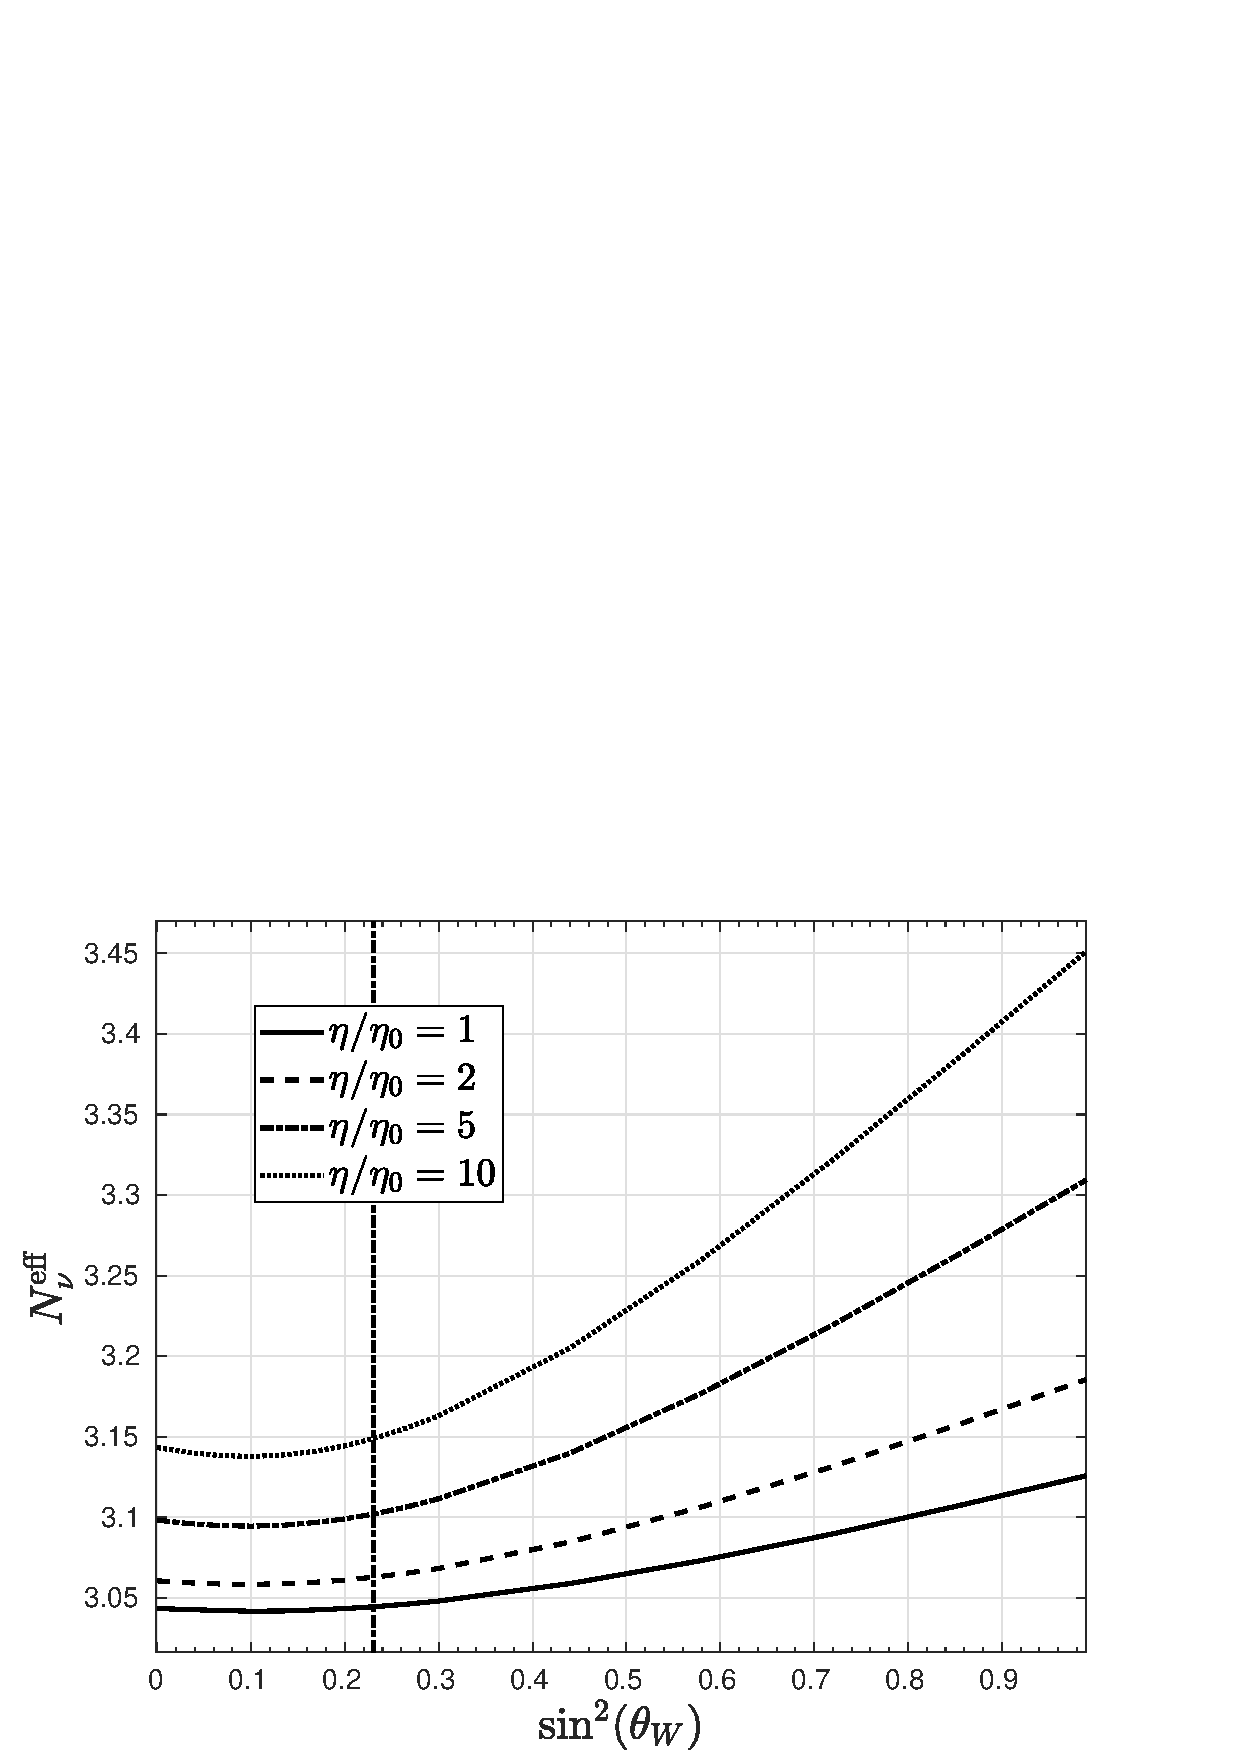
\includegraphics[width=0.90\linewidth]{04-birrell/ParametricStudies/Figures/N_eff2.pdf}}
\caption{Change in effective number of neutrinos $N_\nu^{\mathrm{eff}}$ as a function of Weinberg angle for several values of $\eta/\eta_0=1,2,5,10$. Vertical line is $\sin^2(\theta_W)=0.23$. \radapt{Birrell:2014uka}}
\label{NnuParams} 
 \end{figure}
%%%%%%%%%%%%%%%%%%%%

We performed a least squares fit of $N_\nu^{\mathrm{eff}}$ over the range $0\leq \sin^2(\theta_W)\leq 1$, $1\leq \eta/\eta_0\leq 10$ shown in figure \ref{NnuParams}, obtaining a result with relative error less than $0.2\%$,
\begin{align}
N_\nu^{\mathrm{eff}}=&3.003-0.095\sin^2(\theta_W) +0.222\sin^4(\theta_W ) -0.164\sin^6(\theta_W )\notag\\
+&\sqrt{\frac{\eta}{\eta_0}}\left(0.043+0.011\sin^2(\theta_W) +0.103\sin^4(\theta_W)\right)\,.
\end{align}
$N_\nu^{\mathrm{eff}}$ is monotonically increasing in $\eta/\eta_0$ with dominant behavior scaling as $\sqrt{ \eta/\eta_0}$. Monotonicity is to be expected, as increasing $\eta$ decreases the freeze-out temperature and the longer neutrinos are able to remain coupled to $e^\pm$, the more energy and entropy from annihilation is transferred to neutrinos.

We complement this with fits to the photon to neutrino temperature ratios $ T_\gamma / T_{\nu_e}$, $T_\gamma / T_{\nu_\mu}= T_\gamma / T_{\nu_\tau} $, and the neutrino fugacities, $\Upsilon_{\nu_e}, \Upsilon_{\nu_\mu}=\Upsilon_{\nu_\tau}$, again with relative error less than $0.2\%$, 
\begin{align}
\frac{T_\gamma}{T_{\nu_\mu}}=&1.401+0.015x-0.040x^2+0.029x^3-0.0065y+0.0040xy-0.017x^2y\,, \notag\\
\Upsilon_{\nu_e}=&1.001+0.011x-0.024x^2+0.013x^3-0.005y-0.016xy+0.0006x^2y\,,\notag\\ 
\frac{T_\gamma}{T_{\nu_e}}=&1.401+0.015x-0.034x^2+0.021x^3-0.0066y-0.015xy-0.0045x^2y\,,\notag\\
\Upsilon_{\nu_\mu}=&1.001+0.011x-0.032x^2+0.023x^3-0.0052y+0.0057xy-0.014x^2y\,,
\end{align}
where
\begin{equation}%{align}
x\equiv \sin^2(\theta_W)\, ,\qquad
y\equiv \sqrt{\frac{\eta}{\eta_0}}\,.
\end{equation}%{align}

%%%%%%%%%%%%%%%%%%%%
\begin{figure}
\centerline{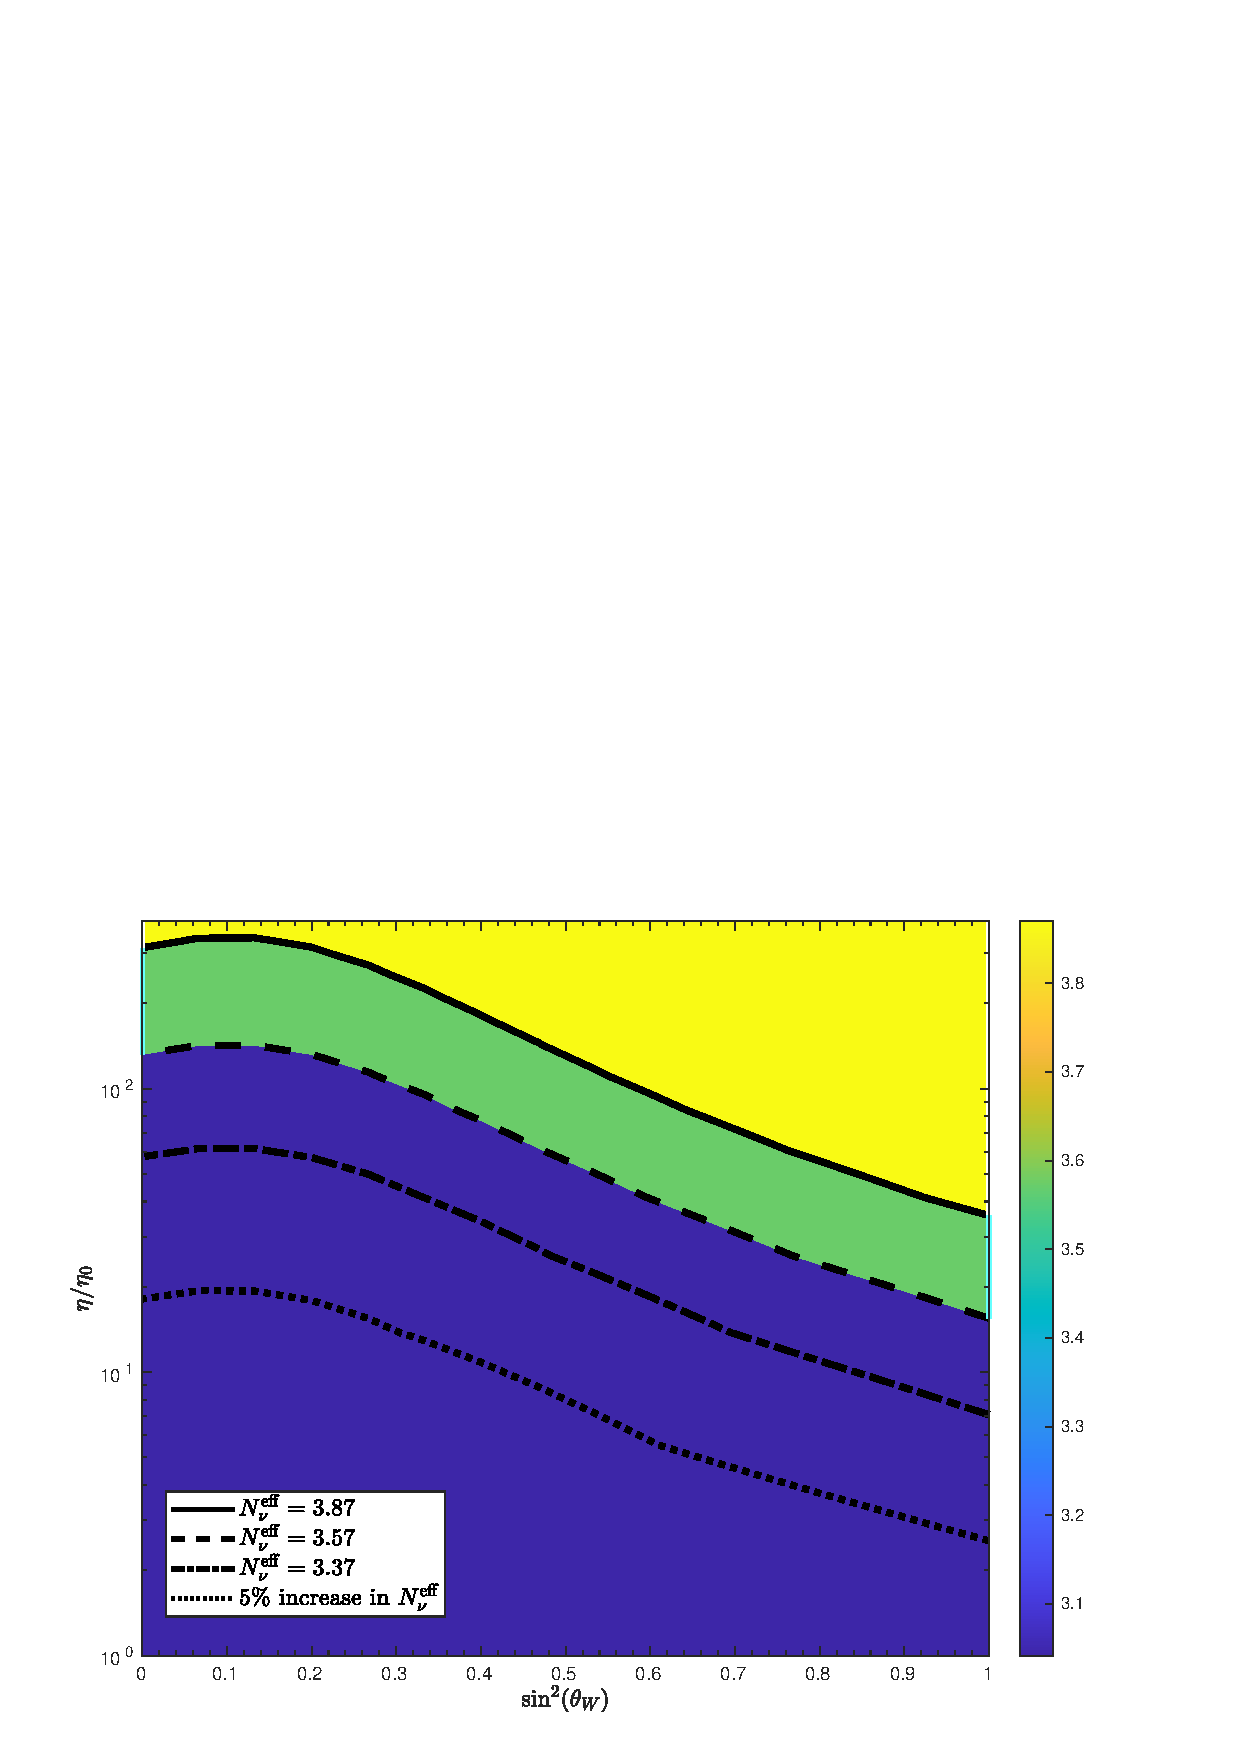
\includegraphics[width=0.99\linewidth]{04-birrell/ParametricStudies/Figures/region_plot_legend.pdf}
}
\caption{$N_\nu^{\mathrm{eff}}$ bounds in the $\eta/\eta_0, \sin^2(\theta_W)$ plane. Blue for $N_\nu^{\mathrm{eff}}\in (3.03,3.57)$ corresponding to Ref.~\cite{Planck:2013pxb} CMB+BAO analysis\index{CMB} and green extends the region to $N_\nu^{\mathrm{eff}}<3.87$ i.e. to CMB+$H_0$. Dot-dashed line delimits the 1 standard-deviation lower boundary of the second analysis. \radapt{Birrell:2014uka}}
\label{NnuDomain}
 \end{figure}
%%%%%%%%%%%%%%%%%%%%

The bounds on $N_\nu^{\mathrm{eff}}$ from the Planck analysis \cite{Planck:2013pxb} can be used to constrain time or temperature variation of $\sin^2(\theta_W)$ and $\eta$. 
In Figure \ref{NnuDomain} the blue region shows the combined range of variation of natural constants compatible with CMB+BAO and the green region shows the extension in the range of variation of natural constants for CMB+$H_0$, both at a $68\%$ confidence level. The dot-dashed line within the blue region delimits this latter domain. The dotted line shows the limit of a 5\% change in $N_\nu^{\mathrm{eff}}$. Any increase in $\eta/\eta_0$ and/or $\sin^2(\theta_W)$ moves the value of $N_\nu^{\mathrm{eff}}$ into the domain favored by current experimental results.

%%%%%%%%%%%%%%%%%%%
We have omitted here a discussion of flavor neutrino oscillations. If it weren't for the differences between the matrix elements for the interactions between $e^\pm$ and $\nu_e$ on one hand and $e^\pm$ and $\nu_\mu,\nu_\tau$ on the other, oscillations would have no effect on the flow of entropy into neutrinos and hence no effect on $N_\nu^{\mathrm{eff}}$, but these differences do lead to a modification of $N_\nu^{\mathrm{eff}}$. In \cite{Mangano:2005cc} the impact of oscillations on neutrino freeze-out\index{neutrino!freeze-out} for the present day measured values of $\theta_W$ and $\eta$ was investigated. It was found that while oscillations redistributed energy amongst the neutrino flavors, the impact on $N_\nu^{\mathrm{eff}}$ was negligible. We have neglected oscillations in our study.

%%%%%%%%%%%%%%%%%%%%%%%%%%%%%%%%%%%%
\para{Primordial Variation of Natural Constants}\index{Natural constants!variation}
We end our study of neutrino freeze-out by exploring what neutrino decoupling in the early Universe can tell us about the values of natural constants when the Universe was about one second old and at an ambient temperature near to 1 MeV (11.6 billion degrees K). Our results were presented assuming that the Universe contains no other effectively massless particles but the three left handed neutrinos and three corresponding right handed anti-neutrinos. 

In \rf{NnuParams} we see that, near the present day value of the Weinberg angle $\sin^2(\theta_W)\simeq 0.23$, the effect of changing $\sin^2(\theta_W)$ on the decoupling of neutrinos is relatively small. The dominant variance is due to the change in the coupling strength $\eta/\eta_0$, \req{etaDef} and \req{eta0Def}. The dotted line in Figure \ref{NnuDomain} shows that in order to achieve a change in $N_\nu^{\mathrm{eff}}$ at the level of up to 5\%, i.e., $N_\nu^{\mathrm{eff}}\lesssim 3.2 $, $\eta/\eta_0$ must change significantly, e.g., increasing by an order of magnitude.

It is not possible to exclude with certainty such a large scale in the primordial Universe as we will now argue considering the natural constants contributing to $\eta$ and their required
modification:
\begin{itemize}
\item
In models of emergent gravity we can imagine a `melting' of gravity in the hot primordial Universe, just like we see the vacuum structure and quark confinement melt. Conversely, and perhaps more attractive in light of the present day interest in the so called Hubble-tension, there could be present-era weakening of gravity which would allow the Universe expansion to accelerate and more generally could also modify the dark energy input into Universe dynamics. Whether such a variable gravity model can be realized will be a topic for future consideration. Considering that $\eta\propto M_p\propto G_N^{-1/2}$ the value of $\eta$ will change in the opposite to the strength of gravity: An order magnitude change in $\eta$ at the time of neutrino decoupling translates into two orders of magnitude (inverse) change in the strength of gravity. One would not think this is a possible scenario mainly because neutrino decoupling occurs at a scale so much different from gravity. The question about temporal variation of gravity strength, along with temperature dependence cannot be as yet addressed in absence of fundamental gravity theory. 
\item
Compared to all other elementary particles the electron mass has an unusually low value. This could imply a more complicated mass origin of the electron when compared to other elementary particles which are drawing their mass by the minimal coupling from the Higgs field\index{Higgs!field} . We studied a strong field mechanism for electron mass melting recently~\cite{Evans:2019zyk}. Since $\eta\propto m_e^3$, electron mass would need to change at the time of decoupling of neutrinos by `only' a factor 2.15 to create an order of magnitude impact on $\eta$. This seems not entirely impossible.
\item
A modification by `only' a factor of 1.8 in the vacuum expectation value (VEV) of the Higgs field $v_0\simeq 246$ GeV controlling the weak interaction coupling $G_\mathrm{F}\propto 1/v^4$ would suffice to alter $\eta$ by an order of magnitude. However, if we allow electron mass to be also Higgs controlled, three powers of $v$ would cancel and a change in $v$ by an order of magnitude near to $T\simeq m_e$ would be required. In either case, given our good understanding of the standard model of particle physics we do not believe that the VEV of the Higgs field could be impacted by the conditions prevailing at the time of neutrino decoupling.
\end{itemize}
To summarize: Gravity, even though it is an effective theory poorly understood at a fundamental level, is governed by the Planck mass scale which is many, many orders of magnitude above scales we are exploring in the epoch of neutrino decoupling. Similarly, the Higgs VEV which controls $G_F$ seems also immutable at the neutrino decoupling temperature, considering the relevant scale being different by a factor of about 500,000. On the other hand, electron mass $m_e$ is `anomalously' small, it is the only elementary scale below the temperature scale of neutrino decoupling, hence it is prone to be modifiable in primordial hot Universe. One can wonder if its small mass is due to an interplay between quantum effects, Higgs coupling and QED interaction. If so the mass would be modifiable at a temperature that is larger than the mass value which is the condition for neutrino decoupling. This therefore could be the cause of a substantial primordial increase in $\eta$, impacting the present day Universe expansion speed through the value of $N_\nu^\mathrm{eff}$.
 
One could further argue that any value of $\sin^2(\theta_W)$ is possible at time of neutrino decoupling, as there is no rational for the vacuum observed symmetry breaking mixing value of $\sin^2(\theta_W)$. However, in the SU(5) model unifying quarks and leptons a natural value $\sin^2(\theta_W)=1/4$ appears. Since this model has been discredited by baryon stability, we could still admit any temperature and/or time dependence of $\sin^2(\theta_W)$. Even so the appearance of a natural $\sin^2(\theta_W)=1/4$ value in the framework of one model could imply that a more realistic model will lead to a similar value.


%%%%%%%%%%%%%%%%%%%%%%%%%%%%%%%%
\subsection{Lepton number and effective number of neutrinos}\label{sec:NeffIntro}

\para{Invisible lepton number: relic neutrinos}
Neutrinos\index{neutrino!effective number} decoupled from the cosmic plasma in the early Universe at a temperature of $T=\mathcal{O}(2\mathrm{MeV})$ and became free-streaming\index{free-streaming}. However, after freeze-out neutrinos still continue to play a significant role in the evolution of the Universe and have a impact on cosmological observations such as Big-Bang Nucleosynthesis (BBN)\index{Big-Bang!BBN}, the Cosmic Microwave Background (CMB)\index{CMB}, and the matter spectrum for large scale structure. This is due to the sensitivity of the Hubble parameter to the total energy density in the Universe. Besides photons, neutrinos are the most abundant species and contribute significantly to the relativistic energy density throughout the early Universe, affecting the Hubble expansion rate significantly. 

The contribution of energy density from the neutrino sector can be described by the effective number of neutrinos $N_{\nu}^{\mathrm{eff}}$, which captures the number of relativistic degrees of freedom for neutrinos as well as any reheating that occurred in the sector after freeze-out. The effective number of neutrino is defined as 
\begin{align}\label{Neff}
N_\nu^{\mathrm{eff}}\equiv\frac{\rho^{\mathrm{tot}}_\nu}{\frac{7\pi^2}{120}\left(\frac{4}{11}\right)^{4/3}T_\gamma^4}\;,
\end{align}
where $\rho_\nu^{\mathrm{tot}}$ is the total energy density in neutrinos and $T_\gamma$ is the photon temperature. $N_\nu^{\mathrm{eff}}$ is defined such that three neutrino flavors with zero participation of neutrinos in reheating during $e^+e^-$ annihilation results in $N_\nu^{\mathrm{eff}}=3$. The factor of $\left(4/11\right)^{1/3}$ relates the photon temperature to the free-streaming neutrinos temperature, under the assumption of zero neutrino reheating after $e^+e^-$ annihilation. The currently accepted theoretical value is $N_\nu^{\mathrm{eff}}=3.046$, after including the slight effect of neutrino reheating \cite{Mangano:2005cc,Birrell:2014uka}. The favored value of $N_\nu^{\mathrm{eff}}$ can be found by fitting to CMB data. In 2013 the Planck collaboration found $N_\nu^{\mathrm{eff}}=3.36\pm0.34$ (CMB only) and $N_\nu^{\mathrm{eff}}= 3.62\pm0.25$ (CMB and $H_0$)~\cite{Planck:2013pxb}.

To explain the experimental value of $N_\nu^{\mathrm{eff}}$, many studies aim to improve the calculation of neutrino decoupling in the early Universe, including exploring the dependence of freeze-out on natural constants~\cite{Birrell:2014uka}, the entropy transfer from $e^+e^-$ annihilation and finite temperature correction~\cite{Dicus:1982bz,Heckler:1994tv,Fornengo:1997wa}, neutrino decoupling with flavor oscillations~\cite{Mangano:2001iu,Mangano:2005cc}\index{neutrino!flavor oscillation}, and investigating nonstandard neutrino interactions \cite{Morgan:1981zy,Fukugita:1987uy,Elmfors:1997tt,Vogel:1989iv,Mangano:2006ar,Giunti:2008ve,Mangano:2006ar}.


The standard cosmological model assumes that the lepton asymmetry $L\equiv  [N_\mathrm{L}-N_{\overline{\mathrm{L}}}] /N_\gamma $  (normalized with the photon number) 
between leptons and anti-leptons is small, similar to the baryon asymmetry $B=[N_\mathrm{B}-N_{\overline{\mathrm{B}}}]/N_\gamma $; most often it is assumed $L=B$. Barenboim, Kinney, and Park~\cite{Barenboim:2016shh,Barenboim:2017dfq} noted that the lepton asymmetry of the Universe is one of the most weakly constrained parameters is cosmology and they propose that models with leptogenesis are able to accommodate a large lepton number asymmetry surviving up to today.  Moreover, the discrepancy between $H_\mathrm{CMB}$ and $H_0$ has increased~\cite{riess2018new,Riess:2018byc,Planck:2018vyg}. The Hubble tension and the possibility that leptogenesis in the early Universe resulted in neutrino asymmetry motivate our study of the dependence of $N_\nu^{\mathrm{eff}}$ on lepton asymmetry, $L$. In our work~\cite{Yang:2018oqg} we consider $L\simeq 1$ and explore how this large cosmological lepton yield relates to the effective number of (Dirac) neutrinos $N^{\mathrm{eff}}_\nu$. 

\para{Relation between the effective number of neutrinos and chemical potential} We consider how neutrinos decouple~\cite{Birrell:2014gea} at a temperature of $T_f\simeq 2\,\mathrm{MeV}$ and are subsequently free-streaming. Assuming exact thermal equilibrium at the time of decoupling, the neutrino distribution can be   written as (see~\cite{Birrell:2012gg} and references therein)
\begin{align}
\label{fnudef}
&f_\nu=\frac{1}{\exp{\left(\sqrt{\frac{E^2-m_\nu^2}{T_\nu^2}+\frac{m^2_\nu}{T^2_f}}-\sigma\frac{\mu_\nu}{T_f}\right)+1}}\;,\qquad T_\nu\equiv\frac{a(t_f)}{a(t)}T_f,
\end{align}
where $\sigma=+1(-1)$ denotes particles (antiparticles) and we define the effective neutrino temperature $T_\nu$  by the red-shifting of momentum in the comoving volume element of the Universe.

Since the freeze-out temperature $T_f\gg m_\nu$ and also neutrino temperature $T_\nu\gg m_\nu$ in the domain of our analysis, we consider the massless limit in Eq.\;(\ref{fnudef}). Under this approximation, the total neutrino energy density can be written as
\begin{align}
\label{EnergyDensity}
\rho_\nu^{\mathrm{tot}}
&=\frac{g_\nu\,T_\nu^4}{2\pi^2}\left[\frac{7\pi^4}{60}+\frac{\pi^2}{2}\left(\frac{\mu_\nu}{T_f}\right)^{\!\!2}+\frac{1}{4}\left(\frac{\mu_\nu}{T_f}\right)^{\!\!4}\right].
\end{align}
Substituting Eq.\;(\ref{EnergyDensity}) into the definition of the effective number of neutrinos\index{neutrino!effective number} Eq.~(\ref{Neff}), we obtain 
\begin{align}
\label{Neff002}
N_\nu^{\mathrm{eff}}\!\!
=\!3\!\left(\frac{11}{4}\right)^{\!\!\frac{4}{3}}\!\!\left(\frac{T_\nu}{T_\gamma}\right)^{\!\!4}\!
\left[1\!+\!\frac{30}{7\pi^2}\!\!\left(\frac{\mu_\nu}{T_f}\right)^{\!\!2} 
\!\!+\frac{15}{7\pi^4}\!\!\left(\frac{\mu_\nu}{T_f}\right)^{\!\!4}\right].
\end{align}
From Eq.\;(\ref{Neff002}) we have for the standard photon reheating ratio $T_\nu/T_\gamma=(4/11)^{1/3}$ \cite{Kolb:1990vq} and degeneracy $g_\nu=3$ (flavor), the relation between the effective number of neutrinos and the chemical potential\index{chemical potential} at freeze-out
\begin{align}
\label{NeffPotential}
N_\nu^{\mathrm{eff}}=3\left[1+\frac{30}{7\pi^2}\left(\frac{\mu_\nu}{T_f}\right)^{\!\!2}+ \frac{15}{7\pi^4} \left(\frac{\mu_\nu}{T_f}\right)^{\!\!4}\right].
\end{align}
To solve the neutrino chemical potential $\mu_\nu/T_f$ as a function of the effective number of neutrinos, we can neglect the $(\mu_\nu/T_f)^4$ term in Eq.\;(\ref{NeffPotential}) because $m_\nu\ll T_f$ and obtain
\begin{align}\label{Solution}
\frac{\mu_\nu}{T_f}=\pm\sqrt{\frac{7\pi^2}{30}\left(\frac{N_\nu^{\mathrm{eff}}}{3}-1\right)}.
%=&\pm \pi\sqrt{\sqrt{1+\frac{7}{15}\left(\frac{N_\nu^{\mathrm{eff}}}{3}-1\right)}-1}%\approx
\end{align}
In Fig.\;\ref{ChemicalPotentialNeff} we plot the free-streaming\index{free-streaming} neutrino chemical potential $|\mu_\nu|/T_f$ as a function of the effective number of neutrinos $N_\nu^{\mathrm{eff}}$. For comparison, the solid (blue) line is the exact solution of $|\mu_\nu|/T_f$ by solving Eq.~(\ref{NeffPotential}) numerically, and the (red) dashed line is the approximate solution Eq.~(\ref{Solution}) by neglecting the $(\mu_\nu/T_f)^4$ in calculation. In the parameter range of interest, we show that the term $(\mu_\nu/T_f)^4$ only contributes $\approx 2\%$ to the calculation and henceforth we neglect it, and use the approximation Eq.\;(\ref{Solution}). 

The SM value of the effective number of neutrinos, $N_\nu^{\mathrm{eff}}=3$, is obtained under the assumption that the neutrino chemical potentials are not essential, {\it i.e.\/}, $\mu_\nu\ll T_f$. From Fig.\;\ref{ChemicalPotentialNeff}, to interpret the literature values $N_\nu^{\mathrm{eff}}=3.36\pm0.34$ (CMB only) and $N_\nu^{\mathrm{eff}}= 3.62\pm0.25$ (CMB and $H_0$), we require $0.52\leqslant\mu_\nu/T_f\leqslant0.69$. These values suggest  a possible neutrino-antineutrino asymmetry at freeze-out, {\it i.e.\/} a difference between the number densities of neutrinos and antineutrinos.

%%%%%%%%%%%%%%%%%%%%%%%%%%%%%%%%%%%%%%%%%%%
\begin{figure}[t]
\begin{center}
\includegraphics[width=0.9\linewidth]{./plots/Chemical_Potential_Neff}
\caption{The free-streaming neutrino chemical potential $|\mu_\nu|/T_f$ as a function of the effective number of neutrinos $N_\nu^{\mathrm{eff}}$. The solid (blue) line is the exact solution and the (red) dashed line is the approximate solution neglecting the $(\mu_\nu/T_f)^4$ term; the maximum difference in the domain shown is about $2\%$. \radapt{Yang:2024ret}}
\label{ChemicalPotentialNeff}
\end{center}
\end{figure}
%%%%%%%%%%%%%%%%%%%%%%%%%%%%%%%%



%%%%%%%%%%%%%%%%%%%%%%%%%%%%%%%%
\para{Dependence of effective number of neutrinos on lepton asymmetry}
We now obtain the relation between neutrino chemical potential and the baryon to lepton ratio. Let us consider the neutrino freeze-out\index{neutrino!freeze-out} temperature $T_f\simeq 2.0$\,MeV; here we treat neutrino freeze-out as occurring instantaneously and prior to $e^+e^-$ annihilation (implying zero neutrino reheating). Comoving lepton (and baryon) number is conserved after the epoch of leptogenesis (baryogenesis, respectively) which precedes the epoch  under consideration in this work ($T\lesssim 2$\;MeV). 

The lepton-density asymmetry $\ell $ at neutrino freeze-out can be written as\index{lepton asymmetry}
\begin{align}
\ell_f \equiv\big(n_e-n_{\overline{e}}\big)_f+\sum_{i=e,\mu, \tau}\big(n_{\nu_i}-n_{\overline{\nu}_i}\big)_f,
\end{align}
where we use the subscript $f$ to indicate that the quantities should be evaluated at the neutrino freeze-out temperature. As a first approximation, here we assume that all neutrinos freeze-out at the same temperature and their chemical potentials are the same; {\it i.e.\/},
\begin{align}
\mu_\nu=\mu_{\nu_e}=\mu_{\nu_\mu}=\mu_{\nu_\tau}.
\end{align}
Furthermore, neutrino oscillation implies that neutrino number is freely exchanged between flavors; {\it i.e.\/}, $\nu_e\rightleftharpoons\nu_\mu\rightleftharpoons\nu_\tau$, and we can assume that all neutrino flavors share the same population. Under these assumptions, the lepton-density asymmetry can be written as
\begin{align}
\label{Lasymmetry}  
\ell_f=\big(n_e-n_{\overline{e}}\big)_f+\big(n_{\nu}-n_{\overline{\nu}}\big)_f,
\end{align}
where the three flavors are accounted for by taking the degeneracy $g_\nu=3$ in the last term. The difference in yield of neutrinos and antineutrinos can be written as
\begin{align}
\label{ExcessNeutrino}
\left(n_\nu-n_{\overline{\nu}}\right)_f=\frac{g_\nu}{6\pi^2}T^3_f\bigg[\pi^2\left(\frac{\mu_\nu}{T_f}\right)+\left(\frac{\mu_\nu}{T_f}\right)^{\!\!3}\bigg].
\end{align}


On the other hand, the baryon-density asymmetry $b$ at neutrino freeze-out is given by
\begin{align}
\label{Basymmetry}
b_f \equiv\big(n_p-n_{\overline{p}}\big)_f+\big(n_n-n_{\overline{n}}\big)_f \approx \big(n_p+n_n\big)_f,
\end{align}
where $n_{\overline{n}}$ and $n_{\overline{p}}$ are negligible in the temperature range we consider here. Taking the ratio $\ell_f/b_f$, using charge neutrality\index{charge neutrality}, and introducing the entropy density\index{entropy!density} we obtain
\begin{align}\label{LfBf}
\left(\frac{\ell_f}{b_f}\right)  
\approx\left(\frac{n_p}{n_B} \right)_f+\left(n_{\nu}-n_{\overline{\nu}}\right)_f \left(\frac{s}{n_B}\right)_f \frac{1}{s_f},\qquad n_B=(n_p+n_n),
\end{align}
where we introduce the notation $n_B$ for the baryon number density. The proton concentration at neutrino freeze-out is given by
\begin{align}
\label{X:proton}
\left(\frac{n_p}{n_B}\right)_f&=\frac{1}{1+(n_n/n_p)_f}=\frac{1}{1+\exp{\big[-\left(Q+\mu_\nu\right)/T_f\big]}},
\end{align}
with $Q=m_n-m_p=1.293\,\mathrm{MeV}$. We neglect the electron chemical potential\index{chemical potential!electron} in the last step because the $e^+e^-$ asymmetry is determined by the proton density, and at energies of order a few MeV, the proton density is small, {\it i.e.\/}, $\mu_e\ll T_f$. 

However, as we will see, for our study of $N_\nu^{\mathrm{eff}}$ we will be interested in the case of a large lepton-to-baryon ratio. From Eq.\;(\ref{X:proton}) it is apparent that this can only be achieved through the second term in Eq.\;(\ref{LfBf}), with the first term then being negligible, as it is smaller than $1$. So we further approximate
\begin{align}\label{LB:ratio}
\left(\frac{\ell_f}{b_f}\right)  
\approx\left(n_{\nu}-n_{\overline{\nu}}\right)_f \left(\frac{s}{n_B}\right)_f \frac{1}{s_f}.
\end{align}
We retained the full expression Eq.\;(\ref{X:proton}) in our above discussion to show that the presence of a chemical potential $\mu_\nu\simeq 0.2\,Q$ could lead to small, perhaps noticeable, effects on pre-BBN proton and neutron abundance. We defer this unrelated discussion to a separate future work. Note that for large $|\mu_\nu|$, Eq.\;(\ref{LB:ratio}) implies that the signs of $\mu_\nu$ and $\ell_f$ are the same. However, for very small $\mu_\nu$ the sign of $\ell_f$ is determined by the interplay between (anti)electrons and (anti)neutrinos; {\it i.e.\/}, there is competition between the two terms in Eq.\;(\ref{Lasymmetry} ).

In general, the total entropy density at freeze-out can be written
\begin{align}
\label{eq:EntropyDensity}
s_f=\frac{2\pi^2}{45}g^s_\ast(T_f)\,T_f^3,
\end{align}
where the $g^s_\ast$ counts the degree of freedom for relativistic particles~\cite{Kolb:1990vq}. At $T_f\simeq 2\mathrm{MeV}$, the relativistic species in the early Universe are photons, electron/positrons, and $3$ neutrino species. We have
\begin{align}
g^s_{\ast}&= g_\gamma+\frac{7}{8}\,g_{e^\pm}+\frac{7}{8}\,g_{\nu\bar{\nu}}\left(\frac{T_\nu}{T_\gamma}\right)^{\!\!3}\bigg[1+\frac{15}{7\pi^2}\left(\frac{\mu_\nu}{T_f}\right)^{\!\!2}\bigg]=10.75+\frac{45}{4\pi^2}\left(\frac{\mu_\nu}{T_f}\right)^{\!\!2}\;,
\end{align}
where the degrees of freedom are given by $g_\gamma=2$, $g_{e^\pm}=4$, and $g_{\nu\bar{\nu}}=6$, and we have $T_\nu=T_\gamma=T_f$ at neutrino freeze-out.

%%%%%%%%%%%%%%%%%%%%%%%%%%%%%%%%%
\begin{figure}
\begin{center}
\includegraphics[width=0.9\linewidth]{./plots/Ratio_BL}
\caption{The ratio $B/|L|$ between the net baryon number and the net lepton number as a function of $N^{\mathrm{eff}}_\nu$: The solid blue line shows $B/|L|$. The vertical (red) dotted lines represent the values $3.36\leqslant N_\nu^{\mathrm{eff}}\leqslant3.62$, which correspond to $1.16 \times 10^{-9}\leqslant B/|L|\leqslant 1.51 \times 10^{-9}$ (horizontal dashed lines). \radapt{Yang:2024ret}}
\label{fig:BLRatio}
\end{center}
\end{figure}
%%%%%%%%%%%%%%%%%%%%%%%%%%%%%%%%%%%%%%%%%%%%%%%%%%%%%%%%%%%%%%%%%%

Finally, since the entropy-per-baryon from neutrino freeze-out up to the present epoch is constant, we can obtain this value by considering the Universe's entropy content today~\cite{Fromerth:2012fe}. For $T\ll1\,\mathrm{MeV}$, the entropy content today is carried by photons and neutrinos, yielding
\begin{align}
\label{NbS}
\left(\frac{s}{n_B}\right)_{t_0}&=\frac{\sum_i\,s_i}{n_B}=\frac{n_\gamma}{n_B}\,\bigg(\frac{s_\gamma}{n_\gamma}+\frac{s_\nu}{n_\gamma}+\frac{s_{\bar{\nu}}}{n_\gamma}\bigg)\;\\
&=\left(\frac{1}{B}\right)_{\!\!t_0}\!\!\left[\frac{s_\gamma}{n_\gamma}+\frac{4}{3T_\nu}\frac{\rho_\nu^{\mathrm{tot}}}{n_\gamma}-\frac{\mu_\nu}{T_f}\left(\frac{n_\nu-n_{\bar{\nu}}}{n_\gamma}\right)\right]_{t_0}\;,
\end{align}
where $t_0$ denotes the present day values, we have $B=n_B/n_\gamma= 0.605\times10^{-9}$ (CMB)~\cite{ParticleDataGroup:2016lqr}\index{CMB} from today's observation. The entropy per particle for a massless boson at zero chemical potential\index{chemical potential} is $(s/n)_{\mathrm{boson}}\approx 3.602$.

Substituting Eq.\;(\ref{ExcessNeutrino}) and Eq.\;(\ref{eq:EntropyDensity}) into Eq.\;(\ref{LB:ratio}) yields the lepton-to-baryon ratio\index{lepton-to-baryon number ratio}
\begin{align}\label{LBratioFinal}
&\frac{L}{B}=\frac{45}{4\pi^4}\frac{\pi^2(\mu_\nu/T_f)+(\mu_\nu/T_f)^3}{10.75+{45}(\mu_\nu/T_f)^2/{4\pi^2}}\left(\frac{s}{n_B}\right)_{\!\!t_0}\;,
\end{align}
in terms of $\mu_\nu/T_f$ which is given by Eq.(\ref{Solution}) and the present day entropy-per-baryon ratio. In Fig.\;\ref{fig:BLRatio} we show the ratio between the net baryon number and the net lepton number as a function of the effective number of neutrino species $N^{\mathrm{eff}}_\nu$ with the parameter $ B|_{t_0} =0.605\times 10^{-9}$(CMB). We find that the values $N_\nu^{\mathrm{eff}}=3.36\pm0.34$ and $N_\nu^{\mathrm{eff}}= 3.62\pm0.25$ require the ratio between baryon number and lepton number to be $1.16 \times 10^{-9} \leqslant\, B/|L| \leqslant 1.51\times 10^{-9}$. These values are close to the baryon-to-photon ratio $0.57 \times 10^{-9} \leqslant B  \leqslant 0.67\times 10^{-9}$. 


The large lepton asymmetry from cosmic neutrino can also affect the neutron lifespan in cosmic plasma which is one of the important parameter controlling BBN element abundances. 
In general the neutron lifespan dependence on temperature of the cosmic medium. When temperature $T=\mathcal{O}(\mathrm{MeV})$, neutron decay occurs in the plasma of electron/positron and 
 neutrino/antineutrino. Electrons and neutrinos in the background plasma can reduce the neutron decay rate by Fermi suppression to the neutron decay rate. Furthermore, the neutrino background can still provide the suppression after electron/positron pair annihilation becomes nearly complete. In this case,the large neutrino chemical potential from lepton asymmetry would play an important role and needs to be accounted for in the precision study of the neutron lifespan in the cosmic plasma.

 
%%%%%%%%%%%%%%%%%%%%%%%%%%%%
\para{Extra neutrinos from microscopic primordial processes}
We are interested to improve the understanding of the role of neutrinos produced by secondary processes just after neutrinos chemical freeze-out. The continued presence of electron-positron rich plasma until $T=20$\,keV permits the reaction $\gamma\gamma\to e^-e^+\to\nu\bar{\nu}$ to occur even after neutrinos decouple from the cosmic plasma. This suggests the small amount of extra neutrinos can be produced until temperature $T=20$\,keV and can modify the free streaming distribution and the effective number of neutrinos\index{neutrino!effective number}. In this section, we examine the possible source of extra neutrino from electron-positron plasma and develop methods for
future detailed study.

Considering that neutrinos decouple at $T_f=2$\,MeV and become free streaming after freeze-out. The presence of electron-positron plasma environment from $2\,\mathrm{MeV}>T>0.02$\,MeV can allow the following weak reaction to occur:
\begin{align}
\gamma+\gamma\longrightarrow e^-+e^+\longrightarrow \nu+\bar{\nu}.
\end{align}
Given the  thermal reaction rate per volume $R_{\gamma\gamma\to e\overline{e}}$ for reaction $\gamma\gamma\to e\overline{e}$ and $R_{e\overline{e}\to\nu\overline{\nu}}$ for reaction $e\overline{e}\to\nu\overline{\nu}$, then the thermal reaction rate per volume for $\gamma\gamma\to e^-e^+\to\nu\bar{\nu}$ can be written as
\begin{align}
R_{\gamma\to e\to\nu}=R_{\gamma\gamma\to e\overline{e}}\left(\frac{R_{e\overline{e}\to\nu\overline{\nu}}}{R_{\gamma\gamma\to e\overline{e}}+R_{e\overline{e}\to\nu\overline{\nu}}}\right)\approx R_{e\overline{e}\to\nu\overline{\nu}}
\end{align}
In Fig.~\ref{ExtraNeutrinoRate} we plot the thermal reaction rate per volume for relevant reactions as a function of temperature $2\,\mathrm{MeV}>T>0.05\,\mathrm{MeV}$. It shows that the dominant reaction for the process $\gamma\gamma\to e^-e^+\to\nu\bar{\nu}$ is the $e\overline{e}\to\nu\overline{\nu}$ and can be approximated $R_{\gamma\to e\to\nu}=R_{e\overline{e}\to\nu\overline{\nu}}$ in the temperature we are interested in.
%%%%%%%%%%%%%%%%%%%%%%%%%%%%%%%%%%%%%%%%%%%%%%%%%%%%%%%%%%%%%%%%%%
\begin{figure}[ht]
\begin{center}
\includegraphics[width=0.9\linewidth]{./plots/Extra_neutrino_rate_volume}
\caption{The thermal reaction rate per volume as a function of temperature $2\,\mathrm{MeV}>T>0.05\,\mathrm{MeV}$. The dominant reaction for the process $\gamma\gamma\to e^-e^+\to\nu\bar{\nu}$ is the $e\overline{e}\to\nu\overline{\nu}$ and we have $R_{\gamma\to e\to\nu}=R_{e\overline{e}\to\nu\overline{\nu}}$. \radapt{Yang:2024ret}.}
\label{ExtraNeutrinoRate}
\end{center}
\end{figure}
%%%%%%%%%%%%%%%%%%%%%%%%%%%%%%%%%%%%%%%%%%%%%%%%%%%%%%%%%%%%%%%%%%%

Given the thermal reaction rate, the dynamic equation describing the relic neutrino abundance after freeze-out can be expressed as:
\begin{align}\label{ExtraNeutrioEq}
\frac{dn_\nu}{dt}+3Hn_\nu=R_{e\overline{e}\to\nu\overline{\nu}}(T_{\gamma,e^\pm})-R_{\nu\overline{\nu}\to e\overline{e}}(T_\nu),
\end{align}
where $n_\nu$ is the number density of neutrinos and $H$ is the Hubble parameter. The parameter $T_{\gamma,e^\pm}$ is the equilibrium temperature between photons and $e^\pm$ and $T_\nu$ is the temperature for free-streaming\index{free-streaming} neutrinos: 
\begin{align}
T_\nu=\frac{a(t_f)}{a(t)}T_f,
\end{align}
where $T_f$ is the neutrino freeze-out\index{neutrino!freeze-out} temperature. After neutrinos decoupled from the cosmic plasma, we have $T_\nu\neq T_{\gamma,e^\pm}$. This is because
the conservation of entropy, after freeze-out, the relic neutrino entropy is conserved independently and the entropy from $e^+e^-$ annihilation flows solely into photons and reheats the photons' temperature. However, after neutrino freeze-out, extra entropy from electron-positron plasma can still flow into the free-streaming neutrino sector via the reaction $\gamma\gamma\to e^-e^+\to\nu\bar{\nu}$. To describe this novel situation, kinetic theory for entropy production needs to be adapted, a topic we will address in the future. Here we neglect this extra entropy and consider the standard scenario for first approximation.


In Fig.~\ref{DimensionlessRatio} we plot the temperature ratio $T_\nu/T_{\gamma,e^\pm}$, the rate ratio $R_{\nu\overline{\nu}\rightarrow e\overline{e}}/ R_{e\overline{e}\rightarrow\nu\overline{\nu}}$ and $(R_{e\overline{e}\rightarrow\nu\overline{\nu}}-R_{\nu\overline{\nu}\rightarrow e\overline{e}})/ R_{e\overline{e}\rightarrow\nu\overline{\nu}}$ as a function of temperature. It shows that after neutrino freeze-out, the back reaction $\nu\overline{\nu}\rightarrow e\overline{e}$ becomes smaller compared to the reaction $e\overline{e}\rightarrow\nu\overline{\nu}$ as the temperature cools down. This is because as $T_\nu$ cools down, the density of relic neutrinos becomes so low and their energy becomes too small to interact. However, the hot and rich electron-positron plasma can still annihilate into neutrino pairs without any difficulties.
%%%%%%%%%%%%%%%%%%%%%%%%%%%%%%%%%%%%%%%%%%%%%%%%%%%%%%%%%%%%%%%%%
\begin{figure}[ht]
\begin{center}
\includegraphics[width=0.9\linewidth]{./plots/DimensionlessRatio_ExtraNeutrino}
\caption{The temperature ratio $T_\nu/T_{\gamma,e^\pm}$ (blue line), the rate ratio $R_{\nu\overline{\nu}\rightarrow e\overline{e}}/ R_{e\overline{e}\rightarrow\nu\overline{\nu}}$ (red line) and $(R_{e\overline{e}\rightarrow\nu\overline{\nu}}-R_{\nu\overline{\nu}\rightarrow e\overline{e}})/ R_{e\overline{e}\rightarrow\nu\overline{\nu}}$ (green line) as a function of temperature. It shows that the reaction $\nu\overline{\nu}\rightarrow e\overline{e}$ is small compare to the reaction $e\overline{e}\rightarrow\nu\overline{\nu}$ as temperature cooling down. \radapt{Yang:2024ret}.}
\label{DimensionlessRatio}
\end{center}
\end{figure}
%%%%%%%%%%%%%%%%%%%%%%%%%%%%%
%%%%%%%%%%%%%%%%%%%%%%%%%%%%%%%%%%%%%%%%%%%%%%%%%%%

Solving the dynamic equation of neutrino abundance Eq.(\ref{ExtraNeutrioEq}), the general solution can be written as
\begin{align}
n_\nu(T)=n_\mathrm{relic}(T)+n_\mathrm{extra}(T),\qquad T=T_{\gamma,e^\pm},
\end{align}
where $n_\mathrm{relic}$ represents the relic neutrino number density and $n_\mathrm{extra}$ is the extra number density from the $e^\pm$ annihilation. The relic neutrino density is given by
\begin{align}  &n_\mathrm{relic}=n_\nu^0\exp\left(-3\int_{t_i}^t{dt^\prime}H(t^\prime)\right)=n_\nu^0\exp\left(3\int_{T_i}^T\frac{dT^\prime}{T^\prime}(1+\mathcal{F})\right),\\
&n^0_\nu=g_\nu\frac{3\zeta(3)}{4\pi^2}T^3_i,\qquad \mathcal{F}=\frac{T}{3g^\ast_s}\frac{dg^\ast_s}{dT},
\end{align}
where $T_i$ is the initial temperature and $g^\ast_s$ is the entropy degrees of freedom\index{entropy!degrees of freedom}. The extra neutrino density can be written as
\begin{align}
n_\mathrm{extra}=-&\exp\left(3\int_{T_i}^T\frac{dT^\prime}{T^\prime}(1+\mathcal{F})\right)\notag\\
\times&\int_{T_i}^T\frac{dT^\prime}{T^\prime}\frac{R_{e\overline{e}}(T^\prime)-R_{\nu\overline{\nu}}(T^\prime_\nu)}{H(T^\prime)}\left(1+\mathcal{F}\right)\exp\left(-3\int_{T_i}^{T^{\prime}}\frac{dT^{\prime\prime}}{T^{\prime\prime}}(1+\mathcal{F})\right).
\end{align}
%%%%%%%%%%%%%%%%%%%%%%%%%%%%%%%%%%%%%%%%%%%%%%%%%%%%%%%%%%%%%%%%%%
\begin{figure}[ht]
\begin{center}
\includegraphics[width=0.9\linewidth]{./plots/ExtraNeutrinoRatio}
\caption{the ratio between $n_{extra}/n_{relic}$ as a function of temperature with different neutrino freeze-out temperature $T_f$. It shows that the higher freeze-out temperature $T_f$ the higher number of extra neutrinos can be produced. \radapt{Yang:2024ret}.}
\label{ExtraNeutrinoRatio}
\end{center}
\end{figure}
%%%%%%%%%%%%%%%%%%%%%%%%%%%%%%%%%%%%%%%%%%%%%%%%%%%%%%%%%%%%%%%%%%%

In Fig.~\ref{ExtraNeutrinoRatio} we plot the ratio between $n_\mathrm{extra}/n_\mathrm{relic}$ as a function of temperature with different neutrino freeze-out temperature $T_f$. It shows that the number of extra neutrinos depends strongly on the parameter $T_f$. This is because the freeze-out temperature determines the timing of the entropy transfer between $e^\pm$ and photon, which subsequently affects the evolution of temperature ratio between neutrinos and photons in the early Universe. The temperature ratio affects the rate ratio between $\nu\overline{\nu}\to e\overline{e}$ and $ e\overline{e}\to\nu\overline{\nu}$, because once the neutrino is too cold and the back reaction $\nu\overline{\nu}\to e\overline{e}$ can not maintain the balance, the $e^\pm$ annihilation starts to feed the extra neutrinos to the relic neutrino background. 

In addition to the annihilation of electron-positron pairs, there are other sources that can contribute to the presence of extra neutrinos in the early Universe. These additional sources include particle physics phenomena and plasma effects: neutrinos from charged leptons $\mu^\pm,\tau^\pm$ decay, neutrinos from the $\pi^\pm$ decay, and neutrino radiation from massive photon decay in electron-positron rich plasma. All of these potential sources of extra neutrinos can impact the distribution of freely streaming neutrinos and the effective number of neutrinos. Understanding these effects is crucial to comprehending how the neutrino component influences the expansion of the Universe, as well as the potential implications for large-scale structure formation and the spectrum of relic neutrinos.
